\begin{frame}[t]
	\frametitle{Optimization: Dependices}

	For optimization we rely on
	\begin{itemize}
		\item 
\includegraphics[height=1cm]{images/ifopt.png}
		\item 
\includegraphics[height=2cm]{images/Ipopt.png}
	\end{itemize}
\end{frame}


\begin{frame}[fragile]
	\frametitle{Optimization: Interface}
	\begin{columns}
		\begin{column}{0.4\textwidth}
			\begin{lstlisting}[language=python]

waypoints = np.random.rand(4, 2)

c1 = broken_lines_path(waypoints)
c2 = minimum_acceleration_path(waypoints)
c3 = minimum_jerk_path(waypoints)
c4 = minimum_snap_path(waypoints)
c5 = minimum_crackle_path(waypoints)

plot2d_compare([c1, c2, c3, c4, c5], [
            'green', 'blue', 'magenta', 'red', 'black'],
            ['min vel', 'min acceleration', 'min jerk',
            'min snap', 'min crackle'])

    \end{lstlisting}
		\end{column}
		\begin{column}{0.6\textwidth}
			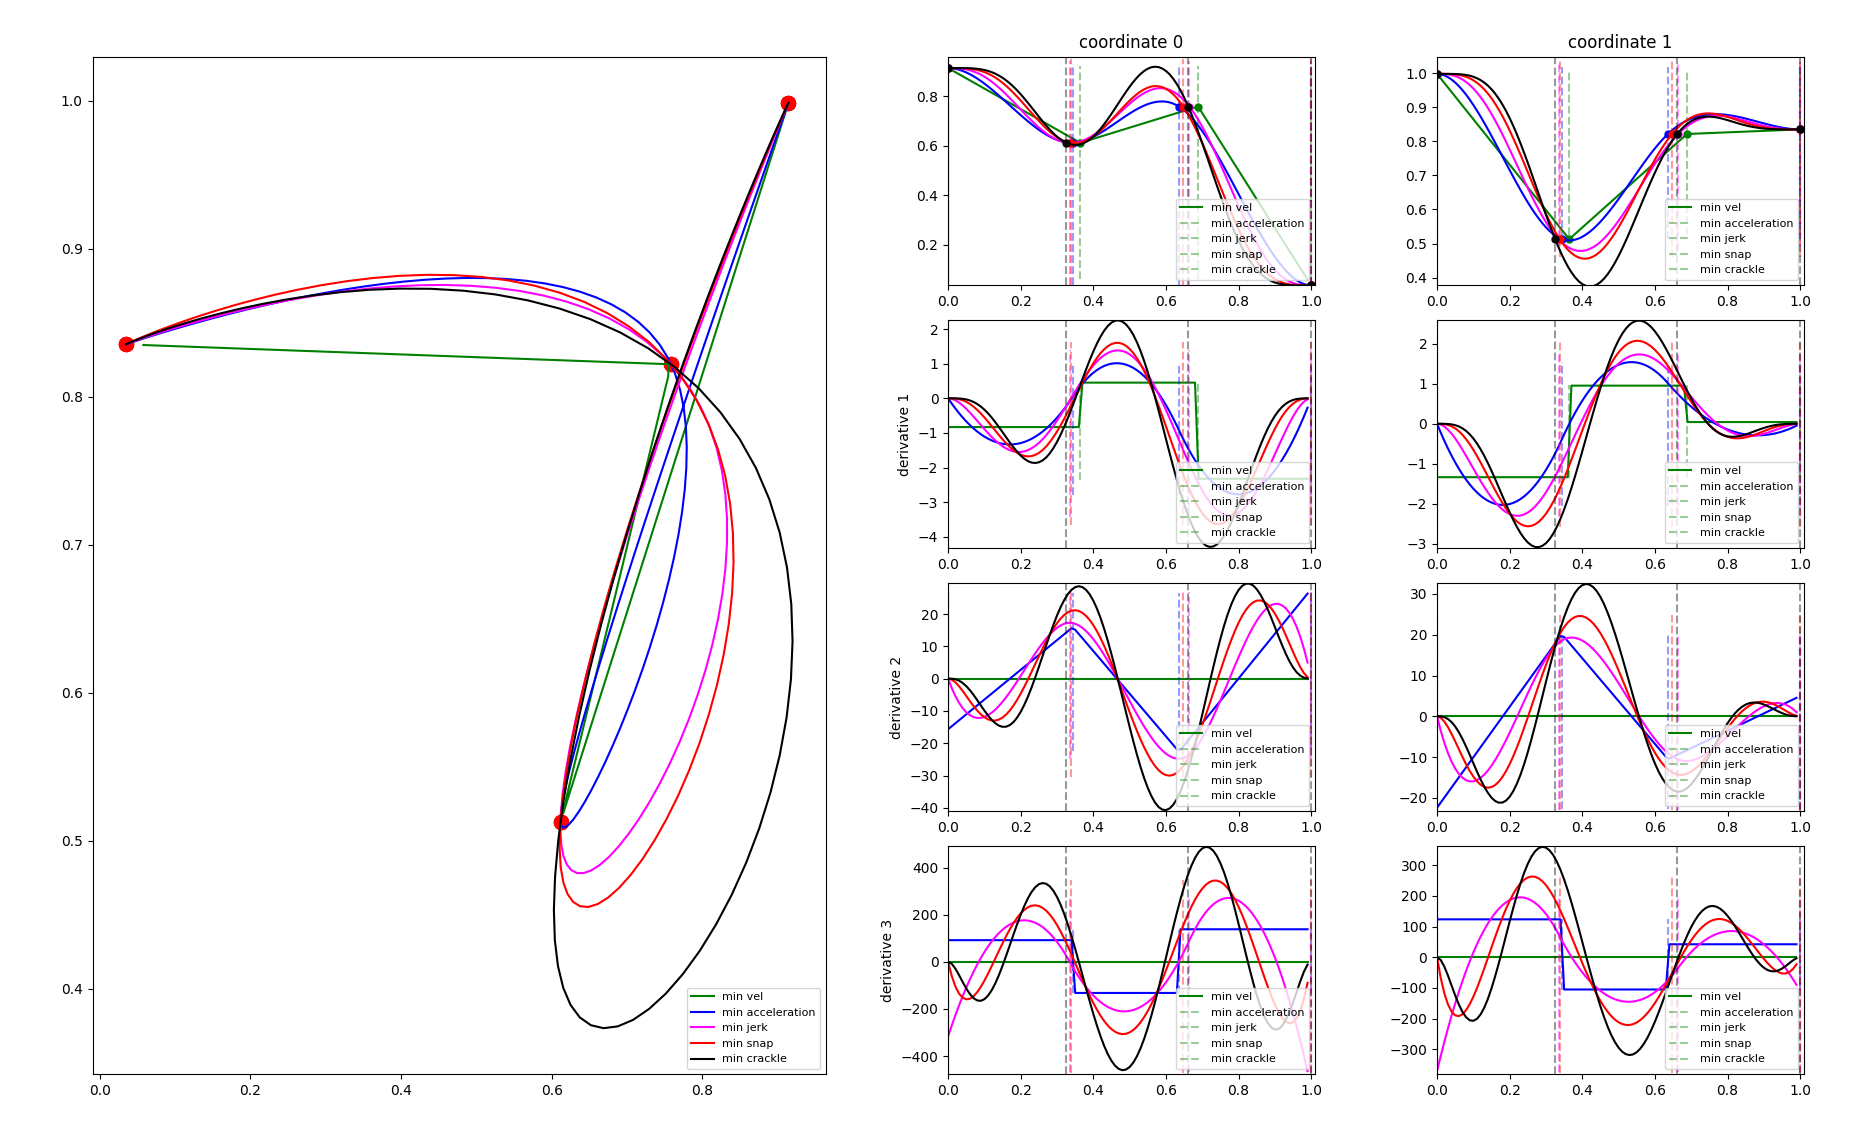
\includegraphics[width=\textwidth]{./images/comparison.png}
		\end{column}
	\end{columns}

\end{frame}
\begin{frame}[fragile]
	\frametitle{Optimization: Interface}
	\begin{columns}
		\begin{column}{0.4\textwidth}
			\begin{lstlisting}[language=python]

waypoints = np.random.rand(4, 2)

c1 = broken_lines_path(waypoints)
c2 = minimum_acceleration_path(waypoints)
c3 = minimum_jerk_path(waypoints)
c4 = minimum_snap_path(waypoints)
c5 = minimum_crackle_path(waypoints)

plot2d_compare([c1, c2, c3, c4, c5], [
            'green', 'blue', 'magenta', 'red', 'black'],
            ['min vel', 'min acceleration', 'min jerk',
            'min snap', 'min crackle'])

    \end{lstlisting}
		\end{column}
		\begin{column}{0.6\textwidth}
			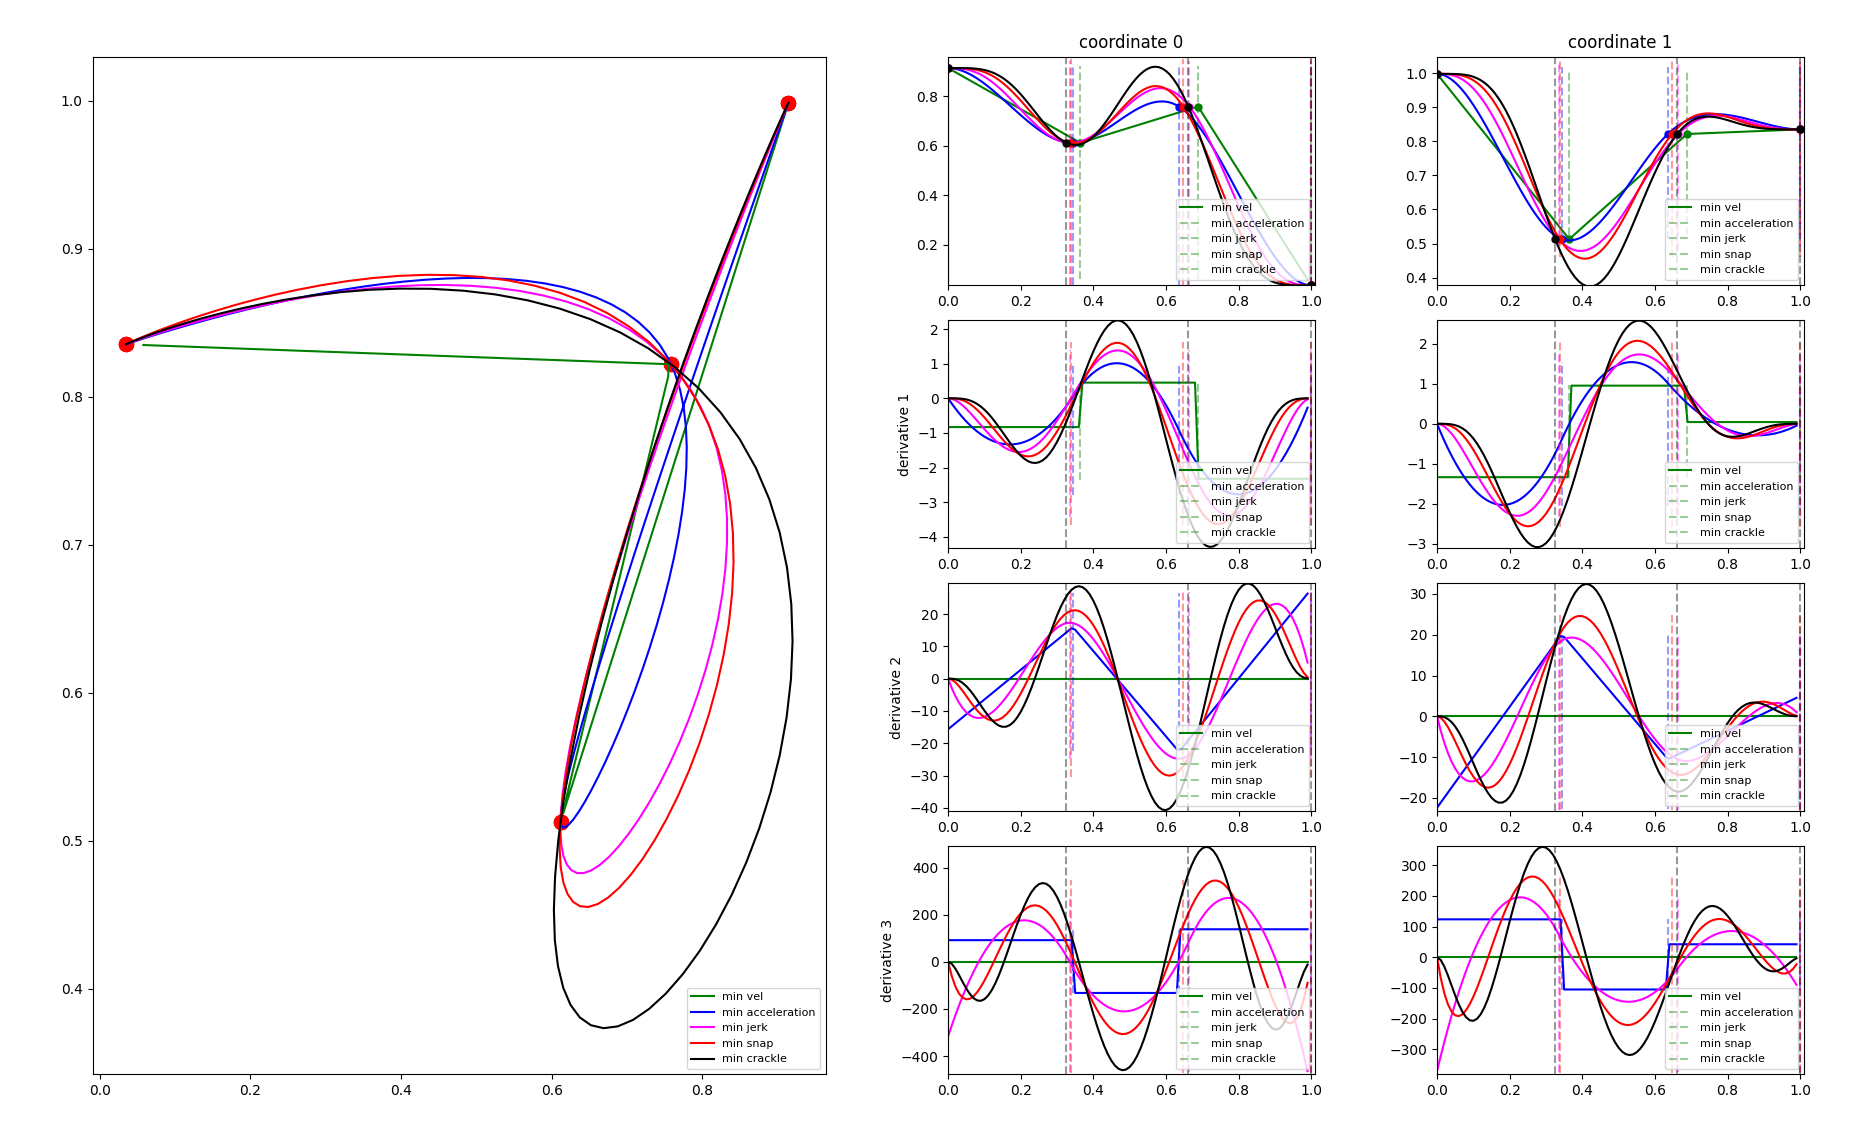
\includegraphics[width=\textwidth]{./images/comparison.png}
		\end{column}
	\end{columns}

\end{frame}
